% !TEX root = ../main.tex

%tools
% \newcommand{\souffle}{\textsc{Souffl\'{e}}\xspace}
% \newcommand{\vampire}{\textsc{Vampire}\xspace}
% \newcommand{\eprover}{\textsc{E}\xspace}
% \newcommand{\spass}{\textsc{Spass}\xspace}

\newcommand{\souffle}{Souffl\'{e}\xspace}
\newcommand{\vampire}{Vampire\xspace}
\newcommand{\eprover}{E\xspace}
\newcommand{\spass}{Spass\xspace}


%languages
% \newcommand{\Datalog}{\textsc{Datalog}\xspace}
\newcommand{\Datalog}{Datalog\xspace}

%datalog notation
% \mathchardef\mhyphen="2D
% \makeatletter
% \newcommand*{\rl}{\mathrel{\texttt{:}\hspace{-0.075em}\mhyphen}}
% \makeatother
\newcommand*{\rl}{\mathrel{\leftarrow}}
\newcommand*{\comma}{\mathrel{\wedge}}

\renewcommand*{\phi}{\varphi}

\newcommand{\typedRel}[1]{\mathit{#1}}
\newcommand{\typed}[2]{\typedRel{#1}({#2})}

% Notation for Horn clauses definitions
\newcommand{\pred}[1]{\mathit{#1}} % predicates
\newcommand{\const}[1]{\mathrm{#1}} % constants
\newcommand{\type}[1]{\mathrm{#1}} % types

\newcommand{\sem}[1]{(#1)} % types

%-------------------------------------------------------------------------------
\section{Introduction}
\label{sect:aws/introduction}
Computer networks are typically built from a variety of specialised heterogeneous devices running complex distributed protocols. Network administrators, responsible for operability of a network, must configure and deploy every protocol separately on each individual device. In an effort to simplify this task, \emph{software-defined networking} (SDN)~\cite{SDN} has been proposed as a modern alternative. SDN provides an layer of software that is installed on each of the network devices and a logically-centralised controller that manages connectivity settings of each device. Administrators can therefore manage networks at a higher level of abstraction by programming them from the controller, typically in a domain specific language~\cite{DBLP:journals/cm/FosterGRSFKMRRSWH13}. The SDN architecture is often credited with flexibility and ease of maintenance compared to traditional networks~\cite{benzekki2016software}.

Modern platforms for cloud computing such as Amazon Elastic Compute Cloud, Google Compute Engine and Azure Virtual Machines offer their users means of configuring \emph{virtual private cloud} (VPC) networks in the style of SDN. Administrators of such networks use a centralised control panel or a specialised API to launch network nodes, set up subnets and route tables, and tune connectivity and security settings of the network. Despite the increase of usability provided by the cloud platforms, VPC networks remain prone to misconfigurations. These misconfigurations are caused by the complexity of large-scale enterprise networks and might lead to downtimes and breaches of security. Discovering such misconfigurations in industrial-sized networks is both labor-intensive and computationally hard. %Therefore, verifying the correctness of network configurations is an important and challenging task.

The presence of a centralised network configuration facilitates automated analysis and synthesis of SDN networks. Indeed, several tools have been developed~\cite{batfish,jayaraman2014automated,DBLP:conf/icdcit/BjornerJ15,DBLP:conf/pldi/BallBGIKSSV14,Veriflow,ConfigChecker,Anteater,DBLP:conf/cav/El-HassanyTVV17} in an effort to verify various SDN components. These tools employ specialised algorithms~\cite{Veriflow} as well as general purpose reasoning engines such as \Datalog~\cite{muZ, DBLP:conf/cav/El-HassanyTVV17,batfish}, BDD~\cite{ConfigChecker}, SMT~\cite{jayaraman2014automated,DBLP:conf/icdcit/BjornerJ15} and SAT~\cite{Anteater,DBLP:conf/pldi/BallBGIKSSV14}.

%
% Problem 1: Size of networks, \Datalog works good in this however certain subproblems are hard for datalog
%
Despite the vast body of available tools, the problem of practical verification of enterprise networks remains a challenge. Firstly, the size and intricacy of modern industrial-sized networks results in very difficult constraint satisfaction problems. While most network verification tools depend on a single constraint solving paradigm, we find that no single solver achieves best performance on all verification problems. Secondly, general purpose solvers are very performance-sensitive to problem encodings. Effective encodings are often a ``black art'' for users, resulting in tedious trial and error for a user without a good understanding of the implementation of the underlying solver.

We are interested in checking properties of VPC networks using complementary constraint solvers. Our ultimate goal is to build a portfolio of constraint solvers that leverages the advantages of different types of solvers on different types of properties. In an effort towards this goal in this work we describe an approach to network verification that relies on automated reasoning for first-order logic. Our plan is to integrate this approach to our ongoing work on the portfolio of solvers.

We consider reachability properties that express whether the network traffic is able to flow between given nodes of a VPC network. The traffic flow in these networks is typically controlled by the rules assigned to various networking components provided by the cloud platform. These components include subnets, route tables, access control lists, internet gateways and others. Let us illustrate these properties using the following example of a VPC network. 
\begin{figure*}[th]
\centering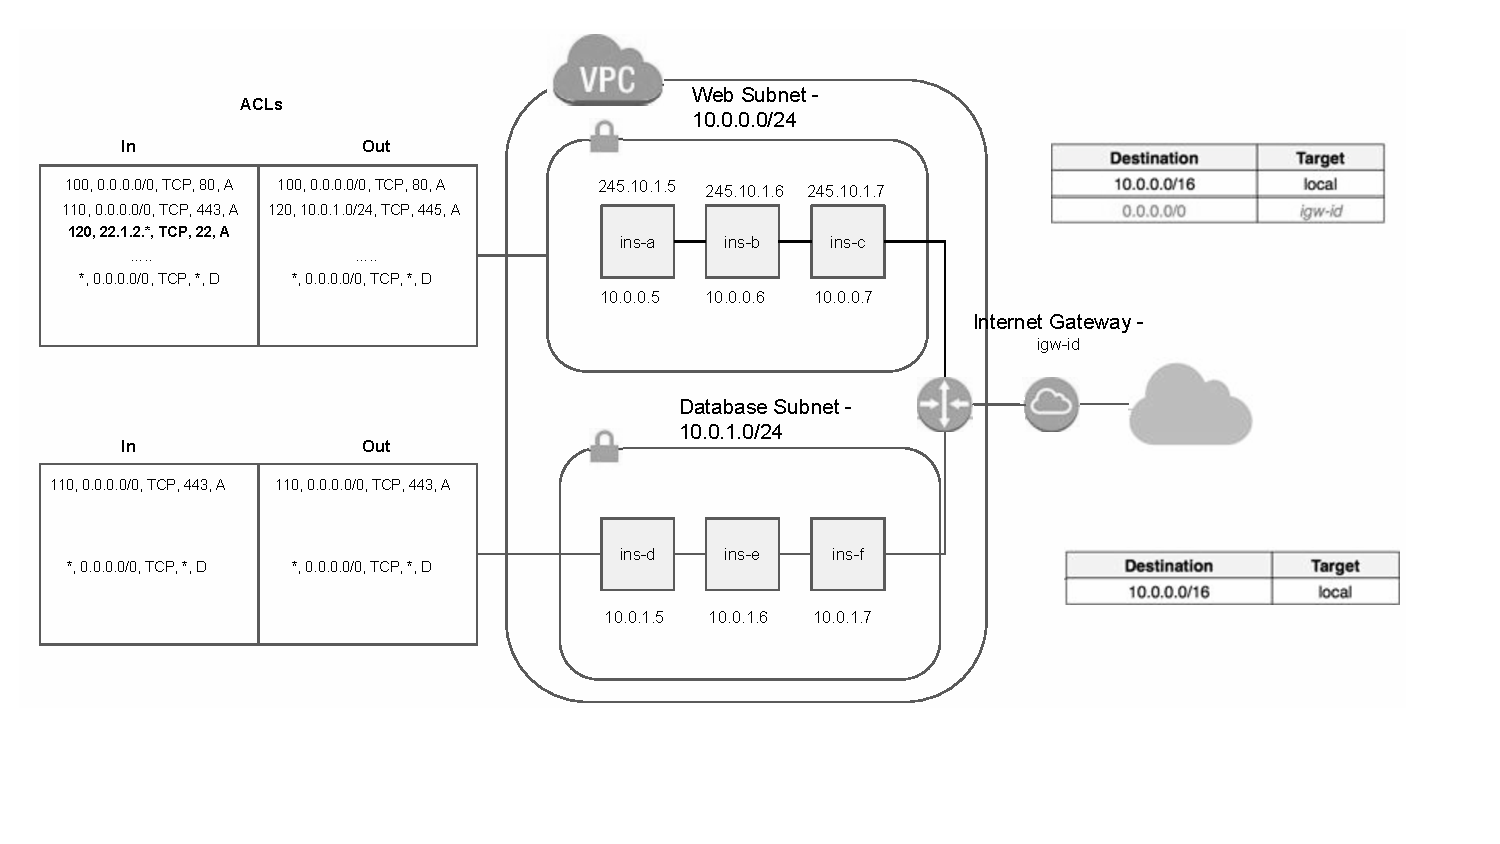
\includegraphics[width=1.0\textwidth]{./aws/fig/vpc2.pdf}
\end{figure*}

This network consists of an internet gateway, two subnets ``Web'' and ``Database'' and three network nodes in each of them. Each of the subnets is assigned with a route table (on the right) and an access control list (ACL, on the left). The route tables allow the network traffic to flow between the subnets and between the ``Web'' subnet and the internet gateway. In other words, the network nodes in the ``Web'' subnet are accessible from the internet, while the nodes in the ``Database'' subnet are not. An ACL consists of rules that filter the network traffic to and from its subnet. In our example, one of the ACL rules of the ``Database'' subnet forbids SSH access to its nodes, both directly and through an intermediate node.

Imagine that this network grows over time and has more nodes and security and access rules added to it. A network administrator may want to make sure that the network retains certain properties after each change in its configuration. For example, the network administrator may want to check the following property.
\begin{example}\label{prop:bool-property}
All network nodes in the subnet ``Web'' can access all network nodes in the subnet ``Database''.
\end{example}

The network administrator might also want to know which networking components satisfy a given property, such as the ones described in the following example.
\begin{example}\label{prop:list-property}
All network nodes that have the port 22 (SSH) accessible from the internet.
\end{example}

We will refer to questions that network administrators might want to answer, such as the ones in Examples~\ref{prop:bool-property} and \ref{prop:list-property}, as \emph{network questions}. In particular, we will refer to questions similar to Example~\ref{prop:bool-property} as \emph{boolean questions}, because an answer to them is ``yes'' or ``no'', and to questions similar to Example~\ref{prop:list-property} as \emph{list questions}, because an answer to them is a list of networking components. Each boolean question can be equivalently phrased as a list question such that the answer to the boolean question is ``yes'' iff the answer to the correspondent list questions is not empty. However, we distinguish these two types of questions because, as we show later, we can more efficiently answer them using different techniques.

Answering network questions manually might be tedious and error-prone in an industrial-size network. For this reason it is necessary to automate this task with specialised tools. In this work we employ automated theorem provers for first-order logic. To this end, we build static models of VPC networks (Section~\ref{sect:aws/specification}), translate these models and network questions about them to problems in first-order logic (Section~\ref{sect:aws/fol}) and check these problems using finite model builders and saturation-based theorem provers (Section~\ref{sect:aws/fol-provers}). In Section~\ref{sect:aws/fol-provers} we argue that finite model builders can more efficiently answer list questions and saturation-based theorem prover can more efficiently answer boolean questions. In Section~\ref{sect:aws/related} we cite related work and in Section~\ref{sect:aws/challenges} we describe the challenges that we faced in this work and outline future work.

\EK{In summary, this paper...}

%-------------------------------------------------------------------------------
\section{Network Reachability Properties}
\label{sect:aws/specification}
We answer network questions statically, that is, instead of sending packets in a network, we build a static model of the network and reason about properties of this model. Our \emph{network model} consists of two parts, the \emph{formal specification} and the \emph{snapshot} of the network. The specification formalises the semantics of each of the components available in the network. For example, the formal specification describes how a route table directs network traffic in a subnet or in which order a firewall applies rules in an access control list. The snapshot describes the topology of the given network. For example, the snapshot contains the list of network nodes, subnets and their route tables. Naturally, the formal specification in the model of each particular VPC network is the same, whereas the snapshot differs. We used models of Amazon VPC networks as part of our ongoing work on network verification using complementary constraint solvers. We express network questions in the language of many-sorted first-order logic. In this section we describe syntax and semantics of network models and network questions.

\subsection{Network Models}
\label{sect:aws/reachability/spec}
A network model is a finite set of first-order Horn clauses expressed in a logic programming style. We disallow function symbols with positive arity and allow stratified negation. We assume the plain logic programming semantics for these Horn clauses, defined in the standard way (see e.g.~\cite{DBLP:books/sp/Lloyd87}). In particular, we make the closed-world assumption and treat negation as failure. In addition, our network models use the theory of bit vectors to describe ports, port ranges, IPv4 addresses and subnet masks.

A \emph{signature} of the network model is a triple $(T, C, P),$ where $T$ is a set of \emph{types}, $C$ is a set of \emph{constants} and $P$ is a set of \emph{predicates}. We assign each constant with a type $\tau\in T$ and each predicate with a type $\tau_1\times\ldots\times\tau_n$ $(n\ge0)$, where $\tau_i\in T$ for each $1\leq i \leq n$. We assume a countable infinite set of \emph{variables}. We assign each variable with a type $\tau\in T$. We call a \emph{term} of the type $\tau\in T$ a constant or a variable of that type. We call an \emph{atom} an expression of the form $p(t_1,\ldots,t_n)$, where $n>0$, $p\in P$ is a predicate of the type $\tau_1\times\ldots\times\tau_n$ and each $t_i$, $1\leq i \leq n$ is a term of the type $\tau_i$. We call a \emph{literal} an atom or its negation.

A \emph{rule} is a Horn clause of the form $A\leftarrow L_1 \wedge \ldots \wedge L_n$ $(n \ge 0)$, where the \emph{head} of the rule $A$ is an atom and each of $L_1,\ldots,L_n$ is a literal. If $n=0$ and all arguments of $A$ are constants then we call such rule a fact. We call a \emph{definition} of the predicate $p \in P$ the set of all rules in the network model that use $p$ in their head.

The specification part of the model contains types, constants, predicates and rules that describe the semantics of the networking components used in the network. For example, the specification defines the semantics of SSH tunneling. One network node can SSH tunnel to another node iff it can either connect to it over SSH directly, or through a chain of one or more intermediate nodes. In order to express this concept, the specification contains predicates $\pred{canSshTunnel}$ and $\pred{canSsh}$, each of the type $\type{node}\times\type{node}$, and the two following rules.
\begin{align*}
\pred{canSshTunnel}(\mathit{Node}_1,\mathit{Node}_2)\leftarrow\:&\pred{canSsh}(\mathit{Node}_1,\mathit{Node}_2). \\
\pred{canSshTunnel}(\mathit{Node}_1,\mathit{Node}_2)\leftarrow\:&\pred{canSshTunnel}(\mathit{Node}_1,\mathit{Node}_3)\\
\wedge\:&\pred{canSshTunnel}(\mathit{Node}_3,\mathit{Node}_2).
\end{align*}
% can-ssh-tunnel-enis: eni * eni
% -: can-ssh-tunnel-enis Eni1 Eni2
% <- can-ssh-enis Eni1 Eni2.
% -: can-ssh-tunnel-enis Eni1 Eni2
% <- can-ssh-tunnel-enis Eni1 Eni3
% <- can-ssh-tunnel-enis Eni3 Eni2.

The snapshot part of the model contains constants and facts that describe the configuration of the networking components in a given network. For example, the snapshot of a network with a single node \verb'i-abcd1234' in a single subnet ``Web'' consists of the constants $\const{node}_\text{abcd1234}$ and $\const{subnet}_\text{Web}$, and the fact $\pred{nodeHasSubnet}(\const{node}_\text{abcd1234},\const{subnet}_\text{Web}).$

We assume that the signature contains
\begin{enumerate*}[label=(\roman*)]
  \item types $\type{bits16}$ and $\type{bits32}$;
  \item $2^{16}$ constants of the type $\type{bits16}$;
  \item $2^{32}$ constants of the type $\type{bits32}$;
  \item predicates $\pred{bits16}_{\le}$ and $\pred{bits16}_{\ge}$ of the type $\type{bits16} \times \type{bits16}$ with a special semantics; and
  \item predicate $\pred{bits32}_\wedge$ or the type $\type{bits32}\times\type{bits32}\times\type{bits32}$ with a special semantics.
\end{enumerate*}
$\type{bits16}$ and $\type{bits32}$ represent the types of 16-bit and 32-bit vectors. The semantics of the predicates is that of the correspondent operations over bit vectors defined in the standard way.

The network specification uses 16-bit vectors to encode port numbers (as integers between 0 and 65535) and port ranges, and 32-bit vectors to encode IPv4 addresses and subnet masks. Port ranges are represented using the type $\type{portRange}$ and the predicate $\pred{portRange}$ of the type $\type{portRange}\times\type{bits16}\times\type{bits16}$. For example, the port range 0--1023 is represented as the constant $\const{portRange}_\text{0--1023}$ of the type $\type{portRange}$ and the fact $\pred{portRange}(\const{portRange}_\text{0--1023},\allowbreak\const{bits16}_0,\allowbreak\const{bits16}_{1023})$, where $\const{bits16}_0$ and $\const{bits16}_{1023}$ are constants of the type $\type{bits16}$. The network specification contains the following definition of the predicate $\pred{portRangeOverlap}$ of the type $\type{portRange}\times\type{portRange}$ that holds when two port ranges overlap.
\begin{equation*}
  \begin{aligned}
\pred{portRangeOverlap}(\mathit{Range}_1,\mathit{Range}_2)\leftarrow\:&\:\pred{portRange}(\mathit{Range}_1,\mathit{From}_1,\mathit{To}_1) \\
  \wedge\:&\:\pred{portRange}(\mathit{Range}_2,\mathit{From}_2,\mathit{To}_2) \\
  \wedge\:&\:\pred{bits16}_\le(\mathit{From}_1,\mathit{To}_2) \\
  \wedge\:&\:\pred{bits16}_\le(\mathit{From}_2,\mathit{To}_1).
  \end{aligned}
\end{equation*}

Finally, we assume that for each type $\tau\in T$ the signature contains the equality predicate $\pred{=}_\tau$ of the type $\tau\times\tau$ and the network model contains the rule $\pred{=}_\tau(X,X)$.

The specification of Amazon~VPC networks that we used in this work consists of approximately 50 types, 200 predicates and over 240 rules.

%\EK{Mention how large network snapshots get?}

\subsection{Network Questions}
\label{sect:aws/reachability/properties}

We express network questions as formulas of many-sorted first-order logic with the standard logical connectives $\vee$, $\wedge$, $\Rightarrow$, $\Leftrightarrow$, $\oplus$ and equality. These formulas only use types, constants and predicates from the signature of the network model. The formulas do not use any function symbols. We allow interpretation of these formulas to use empty domains and otherwise assume the standard semantics of many-sorted first-order logic.

We express boolean questions as closed formulas, that is, formulas in which all variables are bound by a quantifier. Conversely, we express list questions as formulas with free variables. The answer to a boolean question is ``yes'' iff its correspondent formula is valid. The answer to a list question is the set of substitutions of free variables with constants that satisfy its correspondent formula.

Formula~\ref{eq:bool-property} expresses the boolean question in Example~\ref{prop:bool-property}.
\begin{equation}\label{eq:bool-property}
\begin{aligned}
&(\forall w:\type{node})(\forall d:\type{node})\\
&\quad(\pred{nodeHasSubnet}(w, \const{subnet}_\text{Web})\:\wedge\:\\
&\quad\,\,\,\pred{nodeHasSubnet}(d, \const{subnet}_\text{Database}) \Rightarrow~\\
&\quad\,\,\,\quad\pred{nodeCanConnectToNode}(w,d))
\end{aligned}
\end{equation}
% true: all W D: (atom/instance-subnet(W, subnet/web) &&
% atom/instance-subnet(D, subnet/database)) =>
% instance-can-connect-to-instance(W, D).
%In this formula predicates $\pred{instanceHasSubnet}$ and $\pred{instanceCanConnectToInstance}$, and constants $\const{subnet}_\text{Web}$ and $\const{subnet}_\text{Database}$ are part of the signature of the network model~--- the predicate are available in the specification, and the constants are available in the snapshot.

% \EK{We illustrate this difference with the following property.
% \[
% (\forall \mathit{eni}:\type{eni})(\pred{eniOk(\mathit{eni})\vee\neg\pred{eniOk}(\mathit{eni})})
% \]
% % all Eni: (eni-ok(Eni) || !eni-ok(Eni))
% If this query was a formula in first-order logic, it would be a tautology. However, we interpret the property as true iff there exists at least one ENI in the network, that is, if the $\type{eni}$ type is inhabited by at least one value.}

Formula~\ref{eq:list-property} expresses the list question in Example~\ref{prop:list-property}. In this formula $n$ of the type $\type{node}$ and $e$ of the type $\type{eni}$ are free variables.
\begin{equation}\label{eq:list-property}
\begin{aligned}
&\pred{nodeHasEni}(n,e)\:\wedge~\\
&\begin{aligned}
   \pred{reachablePublicTcpUdp}(&\const{dir}_\text{ingress}, \const{proto}_6, e, \const{port}_{22},\\
                                &\const{publicIp}_\text{8:8:8:8}, \const{port}_\text{40000})
 \end{aligned}
\end{aligned}
\end{equation}
% list: instance-has-eni(Instance, Eni) &&
%         reachable-public-tcp-udp(dir/ingress, proto/6,
%                                          Eni, port/22,
%                                          public-ip/8-8-8-8, port/40000).

All predicates and constants used in Formulas~\ref{eq:bool-property} and \ref{eq:list-property} are part of the signature of the network model. Constants $\const{subnet}_\text{Web}$ and $\const{subnet}_\text{Database}$ are part of the network snapshot, and all other predicates and constants are part of the network specification.

% %-------------------------------------------------------------------------------
% \section{Checking Properties with \Datalog}
% \label{sect:aws/datalog}
% We answer a network question by translating the network model and the network question to a \Datalog program and then running it using the \Datalog engine \souffle\cite{souffle}. A \Datalog program consists of a \Datalog \emph{query} and a finite set of \Datalog \textit{rules}. We obtain a query from the network question and a set of rules from both the network model and the network question. We assume that each \Datalog rule has the standard form $A\rl L_1\comma\ldots\comma L_n$ $(n\ge0)$, where $A$ is an atom and each of $L_1,\ldots,L_n$ is a literal, and a \Datalog query has the form $L_1\comma\ldots\comma L_n$ $(n\ge0)$, where each of $L_1,\ldots,L_n$ is a literal. We also assume that all \Datalog rules use stratified negation.

% Network specification is intentional database, network snapshot is extensional database.

\souffle accepts definitions of typed relations, contains the predefined symbol and numeric types, and accepts definitions of new types. The types in \souffle are interpreted under the open-world assumption. We model the types of the network models, interpreted as finite domains, using \Datalog relations with one argument. Let $\tau$ be a type and $c_1,\ldots,c_n$ ($n\ge0$) be constants of this type. We introduce a relation $\typedRel{\tau}$ and add the facts $\typed{\tau}{c_i}$, $1\le i\le n$ to the set of \Datalog rules. We use literals of the form $\typed{\tau}{t}$ in every \Datalog rule to guard the argument $t$ of the type $\tau$ in the head of the rule. % Mention that we can simplify it and only use typing literals near negations.

Let $p(t_1,\ldots,t_n)\leftarrow L_1\wedge\ldots\wedge L_m$ $(n\ge0,m\ge0)$ be a rule in the network model, where $p$ is a predicate of the type $\tau_1\times\ldots\times\tau_n$ and each of $L_1,\ldots,L_m$ is a literal. We translate $p$ to a \Datalog relation $r$ and translate this rule to the \Datalog rule $$r(t_1,\ldots,t_n)\rl\typed{\tau_1}{t_1}\comma\ldots\comma\typed{\tau_n}{t_n}\comma L_1\comma\ldots\comma L_m.$$

We translate a network question expressed as a first-order formula $\phi$ without function symbols to a \Datalog query and a set of \Datalog rules. We start by converting $\phi$ to a prenex disjunctive normal form that is $$(\forall x_1:\tau_1)\ldots(\forall x_n:\tau_n)(\exists y_1:\sigma_1)\ldots(\exists y_m:\sigma_m)(C_1\vee\ldots\vee C_k),$$ where $n\ge0$, $m\ge0$, $k\ge0$, and each of $C_1,\ldots,C_k$ is a conjunction of literals. Let $z_1:\upsilon_1,\ldots,z_l:\upsilon_l$ be all free variables of $\phi$. $l=0$ for formulas expressing boolean network questions and $l>0$ for formulas expressing list network question. We introduce two fresh relations $r$ and $q$ of the types $\tau_1\times\ldots\times\tau_n\times\upsilon_1\times\ldots\times\upsilon_l$ and $\upsilon_1\times\ldots\times\upsilon_l$, respectively. The translated set of \Datalog rules consists of $k+1$ rules: $k$ rules of the form
\begin{align*}
r(x_1,\ldots,x_n,z_1,\ldots,z_l)\rl\;&\typed{\tau_1}{x_1}\comma\ldots\comma\typed{\tau_n}{x_n}\comma~\\
                                     &\typed{\upsilon_1}{z_1}\comma\ldots\comma\typed{\upsilon_l}{z_l}\comma C_i
\end{align*}
for each $1\le i\le k$ and the rule
\begin{align*}
q(z_1,\ldots,z_l)\rl\typed{\upsilon_1}{z_1}\comma\ldots\comma\typed{\upsilon_l}{z_l}\comma\neg r(x_1,\ldots,x_n,z_1,\ldots,z_l).
\end{align*}
Note that we can use each conjunction $C_i$ in a \Datalog rule because each literal in $C_i$ only contains variables and constants~--- there are no function symbols in $\phi$ and they do not appear during a conversion to prenex disjunctive normal form. Finally, the \Datalog query is $\neg q(z_1,\ldots,z_l)$.

% Explain why negations are needed.

We translate types $\type{bits16}$ and $\type{bits32}$ to numeric types for 32 and 16-bit integers, respectively, and translate the predicates over bit vectors into their correspondent built-in \souffle operations.

We illustrate our translation using examples from Section~\ref{sect:aws/motivation}. We translate Formula~\ref{eq:bool-property} that expresses a boolean network question to the \Datalog rules
\begin{align*}
r(W,D)\rl\;& \typed{instance}{W}\wedge\neg\pred{instanceHasSubnet}(W,\const{subnet}_\text{Web}).\\
r(W,D)\rl\;& \typed{instance}{D}\wedge\neg\pred{instanceHasSubnet}(D,\const{subnet}_\text{Database}).\\
r(W,D)\rl\;& \typed{instance}{W}\wedge\typed{instance}{D}\:\wedge\:\\
           & \pred{instanceCanConnectToInstance}(W,D).\\
q\rl\;& \neg r(W,D).
\end{align*}
and the \Datalog query $\neg q$. Note that multiple rules in the definition of $r$ appear because of the translation to disjunctive normal form. We translate Formula~\ref{eq:list-property} that expresses a list network question to the \Datalog rules
\begin{align*}
r(I,E)\rl\;& \typed{instance}{I}\wedge\typed{eni}{E}\:\wedge\:\\
           & \pred{instanceHasEni}(I,E)\:\wedge\:\\
           &\begin{aligned}
               \pred{reachablePublicTcpUdp}(&\const{dir}_\text{ingress},\const{proto}_6,E,\const{port}_{22},\\
                                            &\const{publicIp}_\text{8:8:8:8},\const{port}_\text{40000}).
             \end{aligned}\\
q(I,E)\rl\;& \typed{instance}{I}\wedge\typed{eni}{E}\wedge\neg r(I,E).
\end{align*}
and the \Datalog query $\neg q(I,E)$.

%For example, consider a list query expressed by the formula $(\forall x:\tau)(\exists y:\sigma)(r(x, y) \wedge g(y))$, where $r$ and $g$ are predicates in the network model. We translate it to a \Datalog relation $p$ of the type $\tau\times\sigma$ and a nullary \Datalog relation $q$, two \Datalog rules $p(X,Y)\rl r(X,Y)\comma g(Y)$ and $q\rl \neg p(X,Y)$, and a \Datalog query $\neg q$.


%-------------------------------------------------------------------------------
\section{Checking Properties with Theorem Provers}
\label{sect:aws/fol-provers}
% The continuous advances in automated reasoning have made theorem provers into powerful tools capable of efficiently solving problems coming from real world domains. %\EK{FMB might be just as efficient as datalog search, and saturation-based proof search might be more efficient.} 

We translate network models and network questions to problems in first-order logic. Some of these problems use theories. We solve these problems using saturation-based theorem provers and finite model builders. We use the combination of these two types of provers to leverage the strengths of both of them, which we summarize below.

Saturation-based theorem provers such as E~\cite{E13}, Spass~\cite{Spass} or Vampire~\cite{Vampire13} construct proofs of unsatisfiability of first-order problems. To that end, they first convert the input problem into a set of first-order clauses and then try to derive contradiction from it. Theorem provers saturate the search space by inferring new clauses with inference rules such as binary resolution~\cite{Ganzinger01} and superposition~\cite{NieuwenhuisRubio:HandbookAR:paramodulation:2001}. They employ multiple techniques to prune the search space such as simplification orderings, selection functions and redundancy elimination. Saturation-based provers handle theories by adding incomplete first-order theory axioms to the set of clauses and by using specialised inference rules. In addition to that, \vampire implements the AVATAR modulo theories~\cite{DBLP:conf/gcai/RegerB0V16} architecture that relies on an SMT solver for theory-consistent reasoning in the ground subset of the problem. Saturation-based provers are designed to efficiently solve unsatisfiable problems. Given a satisfiable problem, saturation-based provers can in rare cases report satisfiability and output the saturated set of clauses. However, it is usually not possible to reconstruct a model from this set.

Finite model builders (finders) construct finite counter-models of first-order problems. One of the most successful methods for finite model building was pioneered by the finite model builder MACE~\cite{mccune1994davis}. This method iterates over possible domain sizes, for each domain size grounds the first-order problem with this domain, and translates the resulting formula to a SAT problem. If the SAT problem is satisfied, a finite model of the selected size is reconstructed from the SAT model. Finite model builders Gandalf~\cite{Gandalf}, Paradox~\cite{claessen2003new} and Vampire~\cite{VampireFMB} implement the MACE-style method. Finite model builders generally do not support theories with the notable exception of SMT solver CVC4~\cite{CVC4} that integrates model finding techniques into theory reasoning~\cite{CVC4FMB}. Finite model builders are designed to efficiently solve satisfiable problems. Given an unsatisfiable problem, some finite model builders might detect that the problem cannot have infinite models and in such case report unsatisfiability.

We translate
\begin{enumerate*}[label=(\roman*)]
  \item each boolean question to a first-order problem that is unsatisfiable iff the answer to the question is true; and
  \item each list question to a first-order problem such that each of its finite models corresponds to an answer to the network question.
\end{enumerate*}
Table~\ref{fig:fol-answering-questions} summarises how we interpret a solution found by a theorem prover as the answer to the network question. Saturation-based theorem provers generally cannot answer list questions except for the degenerate case when the answer is empty. With this exception, both types of provers are able to answer both types of network questions. 

\begin{table}
  \center
  \begin{tabular}{lll}
    \hline
    Output of a theorem prover & Boolean question & List question \\
    \hline
    Saturation found unsat & yes & empty list \\
    Saturation found sat   & no  & error \\
    FMB found unsat        & yes & empty list \\
    FMB found a model      & no  & list of answers \\
  \end{tabular}
  \caption{Solutions found by saturation-based theorem provers and finite model builders (FMB) interpreted as answers to network questions.}
  \label{fig:fol-answering-questions}
\end{table}

\EK{Explain why the translated formulas only have finite models. Can we use Infinox~\cite{Infinox} to check finite unsatisfiability, i.e. the absence of models with finite domains?}

%Informally speaking, finite model builders can efficiently answer list questions and saturation-based provers can efficiently answer boolean questions. To complement the performance of a finite model builder and a saturation-based prover, we run both of them in parallel on each first-order problem and record the result of the fastest successful run.

We run a finite model builder and a saturation-based prover in parallel on each problem and record the result of the fastest successful run. We expect that in most cases
\begin{enumerate*}[label=(\roman*)]
  \item a boolean question is answered with ``yes'' by the saturation-based prover and with ``no'' by the finite model builder; and
  \item a list question is answered with the empty list by the saturation-based prover and with a non-empty list by the finite model builder.
\end{enumerate*}

In this work we used the \vampire theorem prover both as a saturation-based theorem prover and a finite model builder. Our translation produces problems expressed in a logic supported by \vampire, namely many-sorted first-order logic with equality, extended with the theory of linear integer arithmetic, the theory of arrays~\cite{VampireAndFOOL} and the theory of tuples~\cite{KKV18}. We wrote the problems in the TPTP language~\cite{TPTP}.

Each problem tackled by a saturation-based theorem prover or a finite model builder consists of the first-order formula $\phi$ that expresses the network question and first-order axioms $A_1,\ldots,A_n$ that we translate from the network model. We translate each boolean question to a problem of the form $A_1\wedge\ldots\wedge A_n \Rightarrow \neg\phi$ and each list question to a problem of the form $A_1\wedge\ldots\wedge A_n \wedge (\forall \bar{z})(q(\bar{z})\Leftrightarrow \phi) \Rightarrow (\forall \bar{z})q(\bar{z}),$ where $q$ is a fresh predicate symbol and $\bar{z}$ are fresh free variables of $\phi$. We reconstruct the answer to a list question from the model of the $q$ predicate~--- each substitution of $\bar{z}$ that satisfies $q$ is an answer to the question.

\section{Network Reachability as First-Order Problem}\label{sect:aws/fol}
Our translation of network models to problems in first-order logic consists of translations of types, constants, predicate definitions and theories. We translate types, constants (Section~\ref{sect:aws/fol/types}) and predicate definitions (Section~\ref{sect:aws/fol/predicates}) using Clark completion~\cite{DBLP:conf/adbt/Clark77}. We use specialised translations for the theory of bit vectors (Section~\ref{sect:aws/fol/theories}) because Vampire does not support it.

\subsection{Types and Constants}\label{sect:aws/fol/types}
Let $\tau$ be a type and $c_1,\ldots,c_n$ ($n\ge0$) be constants of this type. If $n>0$ then we introduce a sort $\tau$, constants $c_1,\ldots,c_n$ of this sort, the domain closure axiom of the form $(\forall x:\tau)(x=c_1 \vee\ldots\vee x=c_n)$ and the distinct constants axiom of the form of a conjunction of literals $c_i\not=c_j$ for all $1\le i\le n$, $1\le j\le n$ and $i\not=j$. If $n=0$ then we do not introduce any sorts or constants and in our translation of predicate definitions replace each subformula of the form $(\forall x:\tau)\varphi$ with logical truth and each subformula of the form $(\exists x:\tau)\varphi$ with logical falsum.

For example, the signature contains the type $\type{dir}$ and two constants $\const{dir}_\text{ingress}$ and $\const{dir}_\text{egress}$ of this type. $\type{dir}$ represents the direction of a network package. We translate this type to first-order logic as a sort $\mathit{dir}$, two constants $\mathit{ingress}$ and $\mathit{egress}$ of this sort and axioms $(\forall x:\mathit{dir})(x=\mathit{ingress}\vee x=\mathit{egress})$ and $\mathit{ingress}\neq\mathit{egress}$.

% dir: type.
% dir/ingress: dir.
% dir/egress: dir.

\subsection{Predicate Definitions}\label{sect:aws/fol/predicates}
%The definitions of predicates in the specification assume the closed world interpretation. It means that a predicate is satisfied iff at least one of its rules is satisfied. To capture the definition in first-order logic we translate a predicate definition using logical equivalence.

Let predicate $p$ of the type $\tau_1\times\ldots\times\tau_n$ be defined using $k\ge0$ rules. Let $x_1:\tau_1,\ldots,x_n:\tau_n$ be fresh variables. If $k=0$ then we translate the definition of $p$ to the axiom $$(\forall x_1:\tau_1)\ldots(\forall x_n:\tau_n)(\neg p(x_1,\ldots,x_n)).$$ If $k>0$ then we translate the definition of $p$ to the axiom $$(\forall x_1:\tau_1)\ldots(\forall x_n:\tau_n)(p(x_1,\ldots,x_n)\Leftrightarrow R_1\vee\ldots\vee R_k),$$ where each of the formulas $R_1,\ldots,R_k$ are translations of each of the $k$ rules, respectively.

Let a rule be of the form $$p(t_1,\ldots,t_n)\leftarrow L_1\wedge\ldots\wedge L_m,\quad(m\ge0)$$ where $t_1:\tau_1,\ldots,t_n:\tau_n$ are terms. Let $y_1:\sigma_1,\ldots,y_l:\sigma_l$ be variables that occur in either of $L_1,\ldots,L_m$ but not in $p(t_1,\ldots,t_n)$. If $m=0$ then we translate the rule to the formula $x_1=t_1\wedge\ldots\wedge x_n=t_n.$ If $m>0$ then we translate the rule to the formula
\begin{equation*}
\begin{aligned}
&x_1=t_1\wedge\ldots\wedge x_n=t_n\;\wedge(\exists y_1:\sigma_1)\ldots(\exists y_l:\sigma_l)(L_1\wedge\ldots\wedge L_m).
\end{aligned}
\end{equation*}

%The translation of rules can be refined to only include equalities for non-distinct variables in the head of the rule. The details of such modification are straightforward.

For example, consider the following definition of the predicate $\pred{link}$ of the type $\type{node} \times \type{node}$ that encodes the equivalence relation between two $\type{node}$s. The definition of $\pred{link}$ in not present in the network model, but it is illustrative of our translation.
\begin{equation*}
\begin{aligned}
&\pred{link}(X,X).\\
&\pred{link}(X,Y)\leftarrow\pred{link}(Y,X).\\
&\pred{link}(X,Y)\leftarrow\pred{link}(X,Z)\wedge\pred{link}(Z,Y).
\end{aligned}
\end{equation*}
% link: node * node
% -: link X X.
% -: link X Y
% <- link Y X.
% -: link X Y
% <- link X Z
% <- link Z Y.

We translate the definition of $\pred{link}$ as a predicate symbol $\mathit{Link}: \mathit{node} \times \mathit{node}$ and the axiom
\begin{equation*}
\begin{aligned}
&(\forall x:\mathit{node})(\forall y:\mathit{node})\\
&\quad
 \begin{aligned}
  (\mathit{Link}(x,y)\Leftrightarrow\:&x=y\:\vee\:\\
                                      &Link(y,x)\:\vee\:\\
                                      &(\exists z:\mathit{node})(\mathit{Link}(x,z)\wedge\mathit{Link}(z,y))).
 \end{aligned}
\end{aligned}
\end{equation*}

Our translation ignores definitions of equality predicates and instead uses the standard equality in first-order logic. %Our translation ignores (the lack of) definitions of bit vector predicates and instead uses other theories as described in the following section.

\subsection{Theories}
\label{sect:aws/fol/theories}
Our early experiments with translating the theory of bit vectors revealed that the quality of this translation crucially affects the performance of Vampire. This led us to develop and compare multiple translations. In this section we first describe translations of bit vectors that use other theories supported by Vampire. Then, we describe a network model transformation that eliminates theories from network models by precomputing the results of theory operations. Finally, we compare these translations.

\subsubsection*{Translations to Other Theories}
Recall that our network models use
\begin{enumerate*}[label=(\roman*)]
  \item the type $\type{bits16}$ and predicates $\pred{bits16}_{\le}$ (``less or equal''), $\pred{bits16}_{\ge}$ (``greater or equal'') and $\pred{=}_\type{bits16}$, and
  \item the type $\type{bits32}$ and predicates $\pred{bits32}_\wedge$ (bitwise conjunction) and $\pred{=}_\type{bits32}$.
\end{enumerate*}
%These two theories use different predicates, therefore we translate 16-bit and 32-bit vectors differently.
We translate 16-bit vectors to integers and 32-bit vectors to tuples and arrays.

\paragraph{16-bit vectors to integers.}
We translate
\begin{enumerate*}[label=(\roman*)]
  \item the type $\type{bits16}$ to $\mathbb{Z}$,
  \item each of the 16-bit vector constants to an integer constant, and
  \item each of the 16-bit predicates to their correspondent predicate symbol in the theory of linear integer arithmetic.
  \item predicate $\pred{=}_\type{bits16}$ to the standard equality.
\end{enumerate*}
\EK{We are translating uint16 to $\mathbb{Z}$~--- explain why it is sound.}

\paragraph{32-bit vectors to tuples.}
We translate
(i) the type $\type{bits32}$ to the tuple sort $(\mathit{bool},\ldots,\mathit{bool})$ where $\mathit{bool}$ is repeated 32 times,
(ii) each of the 32-bit vector constants to a term $(b_1,\ldots,b_{32})$ of this sort, where each of $b_1,\ldots,b_{32}$ is either $\mathit{true}$ or $\mathit{false}$, and
(iii) predicate $\pred{bits32}_\wedge$ to a predicate defined by the following axiom of bitwise conjunction for boolean tuples.
\begin{equation*}
\begin{aligned}
&(\forall x_1\ldots x_{32}:\bool)(\forall y_1\ldots y_{32}:\bool)(\forall z_1\ldots z_{32}:\bool)\\
&\quad(\mathit{bits32}_\wedge((x_1,\ldots,x_{32}),(y_1,\ldots,y_{32}),(z_1,\ldots,z_{32}))\liff\\
&\quad\quad (z_1\liff x_1\wedge y_1)\wedge\ldots\wedge(z_{32}\liff x_{32}\wedge y_{32}))
\end{aligned}
\end{equation*}
(iv) predicate $\pred{=}_\type{bits32}$ to the standard equality.

\paragraph{32-bit vectors to arrays.}
We translate
(i) the type $\type{bits32}$ to the array sort $\mathit{array}(\mathbb{Z},\mathit{bool})$,
(ii) each of the 32-bit vector constant to a fresh constant $v$ of this sort, defined using the axiom $\mathit{select}(v,1)=b_1\wedge\ldots\wedge\allowbreak\mathit{select}(v, 32)=b_{32},$ where each of $b_1,\ldots,b_{32}$ is either $\mathit{true}$ or $\mathit{false}$, and
(iii) predicate $\pred{bits32}_\wedge$ to a predicate defined by the axiom of bitwise conjunction for arrays of booleans.
\begin{equation*}
\begin{aligned}
&(\forall x:\mathit{array}(\mathbb{Z},\mathit{bool}))(\forall y:\mathit{array}(\mathbb{Z},\mathit{bool}))(\forall z:\mathit{array}(\mathbb{Z},\mathit{bool}))\\
&\quad\begin{aligned}
      (\mathit{bits32}_\wedge(x,y,z)\liff\:&(\mathit{select}(z,1)\liff\mathit{select}(x,1)\wedge\mathit{select}(y,1))\:\wedge\\
      &\quad\ldots\\
      \wedge\:&(\mathit{select}(z,32)\liff\mathit{select}(x,32)\wedge\mathit{select}(y,32)))
      \end{aligned}
\end{aligned}
\end{equation*}
(iv) predicate $\pred{=}_\type{bits32}$ to a predicate defined by the following axiom of equality for 32-element arrays of booleans.
\begin{equation*}
\begin{aligned}
&(\forall x:\mathit{array}(\mathbb{Z},\mathit{bool}))(\forall y:\mathit{array}(\mathbb{Z},\mathit{bool}))\\
&\quad\begin{aligned}
      (\pred{=}_\type{bits32}(x, y)\liff\:&\mathit{select}(x,1)=\mathit{select}(y,1)\:\wedge\\
      &\quad\ldots\\
      \wedge\:&\mathit{select}(x, 32)=\mathit{select}(y,32))
      \end{aligned}
\end{aligned}
\end{equation*}

% \paragraph{Extra optimisation.}
% We discovered that operators over 32-bit vectors are only ever used in the following context:
% \begin{equation*}
% \begin{aligned}
% \pred{=}_{bits32}(&\pred{bits32}_{\wedge}(\mathit{CidrBase}_1,\mathit{CidrMask}), \\
%                   &\pred{bits32}_{\wedge}(\mathit{CidrBase}_2,\mathit{CidrMask}))
% \end{aligned}
% \end{equation*}

% Solution~-- fuse them together. Instead of translating equality and conjunction
% \begin{enumerate}
%   \item introduce a predicate $\mathit{EqMask}: \mathit{cidrBase}\times\mathit{cidrBase}\times\mathit{cidrMask}$;
%   \item translate each term of the form \texttt{bits/32/eq (bits/32/and x m) (bits/32/and y m)} into $\mathit{EqMask}(x, y, m)$, and
%   \item add an axiom for $\mathit{EqMask}$.
% \end{enumerate}

\subsubsection*{Precomputation of Theories}
Our network models use 16-bit vectors to describe port numbers and port ranges and 32-bit vectors to describe IPv4 addresses and subnet masks. Bit vector predicates are only used in the definitions of predicates for network primitives. For example, 16-bit vectors only occur in the definitions of predicates that encode set-theoretic operations over port ranges, such as $\pred{portRangeOverlap}$ mentioned in Section~\ref{sect:aws/reachability/properties}. Definitions of higher level predicates only use these operations over port ranges and never the bit vectors predicates.

We eliminate theories from network models by rewriting the definitions of set-theoretic operations over network primitives with results of precomputation of these operations for all primitives used in the network. For example, we precompute the $\pred{portRangeOverlap}$ predicate in the following way. First, we compute the set $S$ of all pairs of overlapping port ranges among the ones used in the network. This requires a quadratic number of integer comparisons. Then, we use set $S$ to build a definition of $\pred{portRangeOverlap}$ that consists of facts of the form $\pred{portRangeOverlap}(\const{portRange}_X,\const{portRange}_Y)$ where $(X,Y)\in S$. We optimise precomputation of some operations by considering their algebraic properties. For example, $\pred{portRangeOverlap}$ is a reflexive symmetric binary relation and 0--65535 overlaps with any other port range. Therefore, we avoid comparing each port range with itself, comparing two port ranges twice and comparing 0--65535 with other port ranges. Instead, we use the following rules in the definition of $\pred{portRangeOverlap}$.
\begin{equation}\label{eq:aws/port-range-algebraic}
\begin{aligned}
&\pred{portRangeOverlap}(\mathit{Range},\mathit{Range}).\\
&\pred{portRangeOverlap}(\mathit{R}_1,\mathit{R}_2)\leftarrow\pred{portRangeOverlap}(\mathit{R}_2,\mathit{R}_1).\\
&\pred{portRangeOverlap}(\const{portRange}_\text{0--65535},\mathit{Range}).
\end{aligned}
\end{equation}

%Here we describe a transformation that eliminates types and predicates of the theory of bit vectors from a network model. The resulting network model can be translated to plain many-sorted first-order logic without theories.

%The motivation for this transformation lies in the following observation. Port numbers in the network models are represented as 16-bit vectors. While the type of 16-bit vectors describes a domain with $2^{16}$ elements, most networks only use a handful of port numbers anywhere in their configuration. We can drastically decrease the size of the domain

%Notice that many networks only use a limited number of CIDR addresses and ports. We found that we could improve performance by representing a CIDR as finite domain that consists only of CIDRs that are used in the network and pre-compute the results of all operations over CIDRs.

%Before translating the network model to first-order logic we remove the $\pred{portRange}$ predicate from the model and rewrite the definition of $\pred{portRangeOverlap}$ in the following way.

% \begin{equation*}
% \begin{aligned}
% &\pred{portRangeOverlap}(\const{portRange}_\text{0--65535},\const{portRange}_\text{0--65535}).\\
% &\pred{portRangeOverlap}(\const{portRange}_\text{0--65535},\const{portRange}_\text{443--443}).\\
% &\pred{portRangeOverlap}(\const{portRange}_\text{0--65535},\const{portRange}_\text{5432--5432}).\\
% &\pred{portRangeOverlap}(\const{portRange}_\text{0--65535},\const{portRange}_\text{80--81}).\\
% &\pred{portRangeOverlap}(\const{portRange}_\text{0--65535},\const{portRange}_\text{9000--9000}).\\
% &\pred{portRangeOverlap}(\const{portRange}_\text{22--22},\const{portRange}_\text{0--65535}).\\
% &\pred{portRangeOverlap}(\const{portRange}_\text{443--443},\const{portRange}_\text{0--65535}).\\
% &\pred{portRangeOverlap}(\const{portRange}_\text{5432--5432},\const{portRange}_\text{0--65535}).\\
% &\pred{portRangeOverlap}(\const{portRange}_\text{80--80},\const{portRange}_\text{0--65535}).\\
% &\pred{portRangeOverlap}(\const{portRange}_\text{80--81},\const{portRange}_\text{0--65535}).\\
% &\pred{portRangeOverlap}(\const{portRange}_\text{80--81},\const{portRange}_\text{80--80}).\\
% &\pred{portRangeOverlap}(\const{portRange}_\text{80--80},\const{portRange}_\text{80--81}).\\
% \end{aligned}
% \end{equation*}

Consider a network that only uses port ranges 0--65535, 22--22, 443--443, 5432--5432, 80--80 and 80--81 in any of the configurations of its components. We found that it is not uncommon for our networks to use trivial port ranges that span one port number. The definition of $\pred{portRangeOverlap}$ precomputed for this network consists of 12 facts or the rule $\pred{portRangeOverlap}(\const{portRange}_\text{80--80},\const{portRange}_\text{80--81})$ together with the rules (\ref{eq:aws/port-range-algebraic}).

\subsubsection*{Comparison of Translations}
We observed that formulas produced by the translation of 32-bit vectors to tuples are generally easier for \vampire than formulas produced by the translation to arrays. We explain it by the fact that the former end up using a more compact representation of bit vectors in first-order logic. The translation to tuples models a 32-bit vector as a single term, while the translation to arrays models it as conjunction of 32 literals. Furthermore, the translation to tuples uses the standard equality that Vampire supports efficiently, while the translation to arrays uses a heavy equality axiom for 32-element arrays. The compact representation of bit vectors as tuples allows Vampire infer bitwise conjunctions faster.

We observed that formulas produced by the translation with precomputed theories are generally easier for \vampire than formulas produced by any of the translations of bit vectors to other theories. We explain it by the fact that the bulky axioms for bitwise conjunction and equality slow down the proof search, whereas these operations are easy to precompute. Although the precomputation of a theory operation has polynomial complexity, we found that for the networks we used in this study it does not significantly slow down answering network questions. Realistic VPC networks only use a small number of distinct network primitives such as port numbers and IP addresses in any of the configurations of its components and the precomputation for them is not heavy. Furthermore, the precomputation of each theory operation usually involves a simple operation over machine integers that can be performed quickly.

Overall we found the precomputation of theories to be the most efficient strategy for translating our network models. It is also the only applicable strategy for translating network models for Vampire's finite model builder, because it only supports plain many-sorted first-order logic without theories.

%-------------------------------------------------------------------------------
\section{Related Work}
\label{sect:aws/related}

Network verification is an attractive target for automated reasoning tools, some of which we mentioned earlier in Section~\ref{sect:aws/introduction}. In this section we focus on approaches to network verification that are most similar to this work and applications of finite model building and saturation theorem proving to similar problems.

Bj\o{}rner et al.~\cite{DBLP:conf/icdcit/BjornerJ15} checked properties of ACLs, routing tables and Border Gateway Protocol policies in Microsoft Azure networks using SMT solver Z3~\cite{Z3}. To that end \cite{DBLP:conf/icdcit/BjornerJ15} implemented a translation of network properties to quantifier-free logical formulas over bit vectors that is aware of the semantics of network components. In comparison, our translation encodes the complete semantics of a VPC network in the quantified problem solved by the theorem prover. We argue that our approach is more scalable at the expense of having to deal with more difficult problems.

Weidenbach~\cite{Weidenbach99} and Goubault-Larrecq~\cite{DBLP:journals/jcs/Goubault-Larrecq10} used finite model building for first-order logic to check unrechability in security protocols.

\EK{
Lisitsa used superposition to proof reachability \cite{DBLP:conf/atva/Lisitsa10}.
}

% ConfigChecker~\cite{ConfigChecker}~--- verification of ACLs, BDD, CRL symbolic model checking, not SDN though.

%VeriFlow~\cite{Veriflow}~--- checking network-wide invariants in real time, specialised algorithm, verification in the data plane.

%Anteater~\cite{Anteater}~--- data plane verification using SAT.

%CrystalNet~\cite{crystalnet}: Emulation of Large Production Networks

%Synthesis of network configurations using \Datalog~\cite{DBLP:conf/cav/El-HassanyTVV17}.

%-------------------------------------------------------------------------------
\section{Challenges and Future Work}
\label{sect:aws/challenges}
This paper presents a work in progress and some of the challenges that we faced are yet to be overcome. We discuss these challenges in this section and suggest directions for future work. We believe that similar challenges are experienced in other practical applications of automated reasoning in first-order logic.

\paragraph{Good translation to first-order logic.}
Automated theorem provers for first-order logic are known to be sensitive to the encoding of the problem they are solving. To ensure efficient representation of practical problems in a theorem prover, these problems should be encoded using theories and syntactical constructs beyond plain first-order logic. Yet not all automated theorem provers efficiently implement these features. While the Vampire theorem prover used in this work supports many useful theories, we miss a support for the theory of bit vectors. The need to work around this limitation hinders a good translation of our network model to first-order logic. %The lack of support for bit vectors led us to device multiple translations for this theory and experiment with these translations.

%\EK{In addition, theorem provers differ in the extensions of plain first-order logic and theories that they support, so one has to target a logic supported by a specific prover when devising a translation.}

\paragraph{Configuration of theorem provers.}
Automated theorem provers typically offer many settings for configuring proof search. For example, Vampire has dozens of options~\cite{DBLP:conf/cade/Reger0V14} that describe a colossal number of possible proof strategies. There is no proof strategy that would be the best for all kinds of problems, and we found that changing the default options of Vampire might result in a strategy that works better on our problems than the default strategy. At the same time, hand-picking good options is tedious and unintuitive, and there is no way of knowing if a hand-picked strategy will work well on all of our problems. Many modern automated theorem provers rely not on one single strategy, but on a portfolio of strategies, which they try one by one during proof search. Theorem provers typically implement portfolios for existing large collections of problems such as TPTP~\cite{TPTP} and SMT-LIB~\cite{SMT-LIB}. To our knowledge, there is no systematic way of assembling a custom portfolio tailored to a specific class of problems.

% \paragraph{Unpredictable runtime.}
% \EK{When comparing the performance of \Datalog and theorem provers we saw that the performance time of \Datalog grows accordingly to the complexity of the problem. Performance of theorem provers looks unpredictable due to the nature of the saturation-based proof search. It's cool when a seemingly hard problem has an easy solution, not so cool the other way around. We wonder if a theorem proving community has an answer to it.}

\paragraph{Finite domains.}
Our formalisation of VPC networks uses large finite domains to describe the topology of a network and the semantics of its components. While finite domains is good news for finite model builders, saturation-based theorem provers are known to have hard time reasoning with them. Domain closure axioms $(\forall x:\tau)(x=c_1 \vee\ldots\vee x=c_n)$ for large values of $n$ result in long clauses that degrade performance of the prover. A technique for efficient superposition theorem proving with these axioms is discussed e.g. in \cite{HillenbrandWeidenbach13}, but this technique is not implemented in any modern theorem prover.

\paragraph{EPR.}
We translate network models to problems that almost fit into the effectively propositional (EPR) fragment of first-order logic, also called the Bernays-Sch\"onfinkel class. These problems do not use function symbols with positive arity, but skolem functions with positive arity might be introduced during clausification. The satisfiability problem for EPR is decidable and there exist efficient tools that deal with this fragment~\cite{DBLP:conf/birthday/Korovin13}. It is possible to translate our network models to problems in EPR, for example by grounding the existentially-quantified variables. The obvious drawback of this translation is the blowup of the size of the resulting problem. Whether this blowup is mitigated by the efficiency of EPR solvers is an interesting question for future work.

\paragraph{Solver-agnostic network models.}
The work presented in this paper contributes to our ultimate goal of checking network properties with diverse complementary constraint solvers. In order to succesfully use different kinds of constraint solvers we need a formalisation of networks that can be equally efficiently translated to different kinds of constraint satisfaction problems. We find that our current formalisation, written in the logic programming style, is friendly for systems like \Datalog~\cite{Datalog}, but not necessarily for theorem provers for first-order logic. For example, some of the predicates in the specification can be more naturally expressed as functions in full first-order logic rather than translated from their encoding as Horn clauses. Ultimately this bias hinders efficient representation of the problem in first-order logic. Designing a more solver-agnostic formalisation of networks is an important direction of future work.

\paragraph{Evaluation.} In this work we used a small collection of network configurations that we verified using Vampire playing a role of both a saturation-based theorem prover and a finite model builder. We leave for future work experiments with (i) other theorem provers for first-order logic, (ii) other kinds of constraint solvers, (iii) different encodings of network problems as constraint satisfaction problems, and (iv) large collections of real world network configurations.

%-------------------------------------------------------------------------------
\section*{Acknowledgments}
\label{sect:aws/acks}
This work has been partially carried out during the first author's visit to Amazon Web Services. We thank Koen Claessen for his valuable comments on an earlier draft of this paper. The first author was partially supported by the Wallenberg Academy Fellowship 2014 and the Swedish VR grant D0497701.
